% UTF-8 encoding
% Compile with latex+dvipdfmx, pdflatex, xelatex or lualatex
% XeLaTeX is recommanded
\documentclass{article}
\usepackage[UTF8]{ctex}
\usepackage{booktabs}
\usepackage{fancyhdr}
\usepackage{float}
\usepackage{graphicx}
\usepackage{helvet}
\usepackage{hyperref}
\usepackage{tabularx}
\usepackage{xcolor}

\usepackage{listings}
\usepackage{tikz}

\usepackage{makeidx}         % allows index generation
\makeindex

\lstset{frame=tblr,
  rulecolor=\color{lightgray},
  language=Java,
  aboveskip=5mm,
  belowskip=5mm,
  showstringspaces=false,
  columns=flexible,
  basicstyle=\linespread{1.0}\small\ttfamily,
  numbers=none,
  % numberstyle=\tiny\color{gray},
  % keywordstyle=\color{blue},
  % commentstyle=\color{dkgreen},
  % stringstyle=\color{mauve},
  breaklines=true,
  breakatwhitespace=true,
  tabsize=3
}

\usepackage{framed}     % These needed for the code formatter
\usepackage{color}
\usepackage{fancyvrb}

% Use helvetica (sans) by default
\renewcommand{\familydefault}{\sfdefault}

% Greenish links
\hypersetup{
  colorlinks=true,
  linkcolor=blue!50!red,
  urlcolor=blue!50!red
}

\setlength{\headheight}{40pt}
\setlength{\headsep}{0.2in}

\pagestyle{fancy}
\lhead{
\includegraphics[width=0.2\textwidth]{img/logo}}
\chead{SPIDriver 用户指南}
\rhead{\thepage}
\cfoot{\textcopyright \the\year \ \ Excamera Labs}
\renewcommand{\headrulewidth}{0.5pt}
\renewcommand{\footrulewidth}{0.5pt}

\usepackage{array}
\newcolumntype{L}[1]{>{\raggedright\let\newline\\\arraybackslash\hspace{0pt}}m{#1}}
\newcolumntype{C}[1]{>{\centering\let\newline\\\arraybackslash\hspace{0pt}}m{#1}}
\newcolumntype{R}[1]{>{\raggedleft\let\newline\\\arraybackslash\hspace{0pt}}m{#1}}

\usepackage{setspace}

\newcommand{\heavyline}{\specialrule{1pt}{1pt}{1pt}}
\newcommand{\png}[1]{
\begin{figure}[H]
\begin{center}
\includegraphics[width=0.75\textwidth]{#1}
\end{center}
\end{figure}
}
\newcommand{\pngw}[2]{
\begin{figure}[H]
\begin{center}
\includegraphics[width=#2\textwidth]{#1}
\end{center}
\end{figure}
}

\newcommand{\mach}[1]{\texttt{\textbf{#1}}}
\newcommand{\gap}{\vspace{10pt}}


\makeatletter
\def\PY@reset{\let\PY@it=\relax \let\PY@bf=\relax%
    \let\PY@ul=\relax \let\PY@tc=\relax%
    \let\PY@bc=\relax \let\PY@ff=\relax}
\def\PY@tok#1{\csname PY@tok@#1\endcsname}
\def\PY@toks#1+{\ifx\relax#1\empty\else%
    \PY@tok{#1}\expandafter\PY@toks\fi}
\def\PY@do#1{\PY@bc{\PY@tc{\PY@ul{%
    \PY@it{\PY@bf{\PY@ff{#1}}}}}}}
\def\PY#1#2{\PY@reset\PY@toks#1+\relax+\PY@do{#2}}

\expandafter\def\csname PY@tok@gd\endcsname{\def\PY@tc##1{\textcolor[rgb]{0.63,0.00,0.00}{##1}}}
\expandafter\def\csname PY@tok@gu\endcsname{\let\PY@bf=\textbf\def\PY@tc##1{\textcolor[rgb]{0.50,0.00,0.50}{##1}}}
\expandafter\def\csname PY@tok@gt\endcsname{\def\PY@tc##1{\textcolor[rgb]{0.00,0.27,0.87}{##1}}}
\expandafter\def\csname PY@tok@gs\endcsname{\let\PY@bf=\textbf}
\expandafter\def\csname PY@tok@gr\endcsname{\def\PY@tc##1{\textcolor[rgb]{1.00,0.00,0.00}{##1}}}
\expandafter\def\csname PY@tok@cm\endcsname{\let\PY@it=\textit\def\PY@tc##1{\textcolor[rgb]{0.25,0.50,0.50}{##1}}}
\expandafter\def\csname PY@tok@vg\endcsname{\def\PY@tc##1{\textcolor[rgb]{0.10,0.09,0.49}{##1}}}
\expandafter\def\csname PY@tok@m\endcsname{\def\PY@tc##1{\textcolor[rgb]{0.40,0.40,0.40}{##1}}}
\expandafter\def\csname PY@tok@mh\endcsname{\def\PY@tc##1{\textcolor[rgb]{0.40,0.40,0.40}{##1}}}
\expandafter\def\csname PY@tok@go\endcsname{\def\PY@tc##1{\textcolor[rgb]{0.53,0.53,0.53}{##1}}}
\expandafter\def\csname PY@tok@ge\endcsname{\let\PY@it=\textit}
\expandafter\def\csname PY@tok@vc\endcsname{\def\PY@tc##1{\textcolor[rgb]{0.10,0.09,0.49}{##1}}}
\expandafter\def\csname PY@tok@il\endcsname{\def\PY@tc##1{\textcolor[rgb]{0.40,0.40,0.40}{##1}}}
\expandafter\def\csname PY@tok@cs\endcsname{\let\PY@it=\textit\def\PY@tc##1{\textcolor[rgb]{0.25,0.50,0.50}{##1}}}
\expandafter\def\csname PY@tok@cp\endcsname{\def\PY@tc##1{\textcolor[rgb]{0.74,0.48,0.00}{##1}}}
\expandafter\def\csname PY@tok@gi\endcsname{\def\PY@tc##1{\textcolor[rgb]{0.00,0.63,0.00}{##1}}}
\expandafter\def\csname PY@tok@gh\endcsname{\let\PY@bf=\textbf\def\PY@tc##1{\textcolor[rgb]{0.00,0.00,0.50}{##1}}}
\expandafter\def\csname PY@tok@ni\endcsname{\let\PY@bf=\textbf\def\PY@tc##1{\textcolor[rgb]{0.60,0.60,0.60}{##1}}}
\expandafter\def\csname PY@tok@nl\endcsname{\def\PY@tc##1{\textcolor[rgb]{0.63,0.63,0.00}{##1}}}
\expandafter\def\csname PY@tok@nn\endcsname{\let\PY@bf=\textbf\def\PY@tc##1{\textcolor[rgb]{0.00,0.00,1.00}{##1}}}
\expandafter\def\csname PY@tok@no\endcsname{\def\PY@tc##1{\textcolor[rgb]{0.53,0.00,0.00}{##1}}}
\expandafter\def\csname PY@tok@na\endcsname{\def\PY@tc##1{\textcolor[rgb]{0.49,0.56,0.16}{##1}}}
\expandafter\def\csname PY@tok@nb\endcsname{\def\PY@tc##1{\textcolor[rgb]{0.00,0.50,0.00}{##1}}}
\expandafter\def\csname PY@tok@nc\endcsname{\let\PY@bf=\textbf\def\PY@tc##1{\textcolor[rgb]{0.00,0.00,1.00}{##1}}}
\expandafter\def\csname PY@tok@nd\endcsname{\def\PY@tc##1{\textcolor[rgb]{0.67,0.13,1.00}{##1}}}
\expandafter\def\csname PY@tok@ne\endcsname{\let\PY@bf=\textbf\def\PY@tc##1{\textcolor[rgb]{0.82,0.25,0.23}{##1}}}
\expandafter\def\csname PY@tok@nf\endcsname{\def\PY@tc##1{\textcolor[rgb]{0.00,0.00,1.00}{##1}}}
\expandafter\def\csname PY@tok@si\endcsname{\let\PY@bf=\textbf\def\PY@tc##1{\textcolor[rgb]{0.73,0.40,0.53}{##1}}}
\expandafter\def\csname PY@tok@s2\endcsname{\def\PY@tc##1{\textcolor[rgb]{0.73,0.13,0.13}{##1}}}
\expandafter\def\csname PY@tok@vi\endcsname{\def\PY@tc##1{\textcolor[rgb]{0.10,0.09,0.49}{##1}}}
\expandafter\def\csname PY@tok@nt\endcsname{\let\PY@bf=\textbf\def\PY@tc##1{\textcolor[rgb]{0.00,0.50,0.00}{##1}}}
\expandafter\def\csname PY@tok@nv\endcsname{\def\PY@tc##1{\textcolor[rgb]{0.10,0.09,0.49}{##1}}}
\expandafter\def\csname PY@tok@s1\endcsname{\def\PY@tc##1{\textcolor[rgb]{0.73,0.13,0.13}{##1}}}
\expandafter\def\csname PY@tok@sh\endcsname{\def\PY@tc##1{\textcolor[rgb]{0.73,0.13,0.13}{##1}}}
\expandafter\def\csname PY@tok@sc\endcsname{\def\PY@tc##1{\textcolor[rgb]{0.73,0.13,0.13}{##1}}}
\expandafter\def\csname PY@tok@sx\endcsname{\def\PY@tc##1{\textcolor[rgb]{0.00,0.50,0.00}{##1}}}
\expandafter\def\csname PY@tok@bp\endcsname{\def\PY@tc##1{\textcolor[rgb]{0.00,0.50,0.00}{##1}}}
\expandafter\def\csname PY@tok@c1\endcsname{\let\PY@it=\textit\def\PY@tc##1{\textcolor[rgb]{0.25,0.50,0.50}{##1}}}
\expandafter\def\csname PY@tok@kc\endcsname{\let\PY@bf=\textbf\def\PY@tc##1{\textcolor[rgb]{0.00,0.50,0.00}{##1}}}
\expandafter\def\csname PY@tok@c\endcsname{\let\PY@it=\textit\def\PY@tc##1{\textcolor[rgb]{0.25,0.50,0.50}{##1}}}
\expandafter\def\csname PY@tok@mf\endcsname{\def\PY@tc##1{\textcolor[rgb]{0.40,0.40,0.40}{##1}}}
\expandafter\def\csname PY@tok@err\endcsname{\def\PY@bc##1{\setlength{\fboxsep}{0pt}\fcolorbox[rgb]{1.00,0.00,0.00}{1,1,1}{\strut ##1}}}
\expandafter\def\csname PY@tok@kd\endcsname{\let\PY@bf=\textbf\def\PY@tc##1{\textcolor[rgb]{0.00,0.50,0.00}{##1}}}
\expandafter\def\csname PY@tok@ss\endcsname{\def\PY@tc##1{\textcolor[rgb]{0.10,0.09,0.49}{##1}}}
\expandafter\def\csname PY@tok@sr\endcsname{\def\PY@tc##1{\textcolor[rgb]{0.73,0.40,0.53}{##1}}}
\expandafter\def\csname PY@tok@mo\endcsname{\def\PY@tc##1{\textcolor[rgb]{0.40,0.40,0.40}{##1}}}
\expandafter\def\csname PY@tok@kn\endcsname{\let\PY@bf=\textbf\def\PY@tc##1{\textcolor[rgb]{0.00,0.50,0.00}{##1}}}
\expandafter\def\csname PY@tok@mi\endcsname{\def\PY@tc##1{\textcolor[rgb]{0.40,0.40,0.40}{##1}}}
\expandafter\def\csname PY@tok@gp\endcsname{\let\PY@bf=\textbf\def\PY@tc##1{\textcolor[rgb]{0.00,0.00,0.50}{##1}}}
\expandafter\def\csname PY@tok@o\endcsname{\def\PY@tc##1{\textcolor[rgb]{0.40,0.40,0.40}{##1}}}
\expandafter\def\csname PY@tok@kr\endcsname{\let\PY@bf=\textbf\def\PY@tc##1{\textcolor[rgb]{0.00,0.50,0.00}{##1}}}
\expandafter\def\csname PY@tok@s\endcsname{\def\PY@tc##1{\textcolor[rgb]{0.73,0.13,0.13}{##1}}}
\expandafter\def\csname PY@tok@kp\endcsname{\def\PY@tc##1{\textcolor[rgb]{0.00,0.50,0.00}{##1}}}
\expandafter\def\csname PY@tok@w\endcsname{\def\PY@tc##1{\textcolor[rgb]{0.73,0.73,0.73}{##1}}}
\expandafter\def\csname PY@tok@kt\endcsname{\def\PY@tc##1{\textcolor[rgb]{0.69,0.00,0.25}{##1}}}
\expandafter\def\csname PY@tok@ow\endcsname{\let\PY@bf=\textbf\def\PY@tc##1{\textcolor[rgb]{0.67,0.13,1.00}{##1}}}
\expandafter\def\csname PY@tok@sb\endcsname{\def\PY@tc##1{\textcolor[rgb]{0.73,0.13,0.13}{##1}}}
\expandafter\def\csname PY@tok@k\endcsname{\let\PY@bf=\textbf\def\PY@tc##1{\textcolor[rgb]{0.00,0.50,0.00}{##1}}}
\expandafter\def\csname PY@tok@se\endcsname{\let\PY@bf=\textbf\def\PY@tc##1{\textcolor[rgb]{0.73,0.40,0.13}{##1}}}
\expandafter\def\csname PY@tok@sd\endcsname{\let\PY@it=\textit\def\PY@tc##1{\textcolor[rgb]{0.73,0.13,0.13}{##1}}}

\def\PYZbs{\char`\\}
\def\PYZus{\char`\_}
\def\PYZob{\char`\{}
\def\PYZcb{\char`\}}
\def\PYZca{\char`\^}
\def\PYZam{\char`\&}
\def\PYZlt{\char`\<}
\def\PYZgt{\char`\>}
\def\PYZsh{\char`\#}
\def\PYZpc{\char`\%}
\def\PYZdl{\char`\$}
\def\PYZhy{\char`\-}
\def\PYZsq{\char`\'}
\def\PYZdq{\char`\"}
\def\PYZti{\char`\~}
% for compatibility with earlier versions
\def\PYZat{@}
\def\PYZlb{[}
\def\PYZrb{]}
\makeatother



\begin{document}

\newpage
\begin{center}
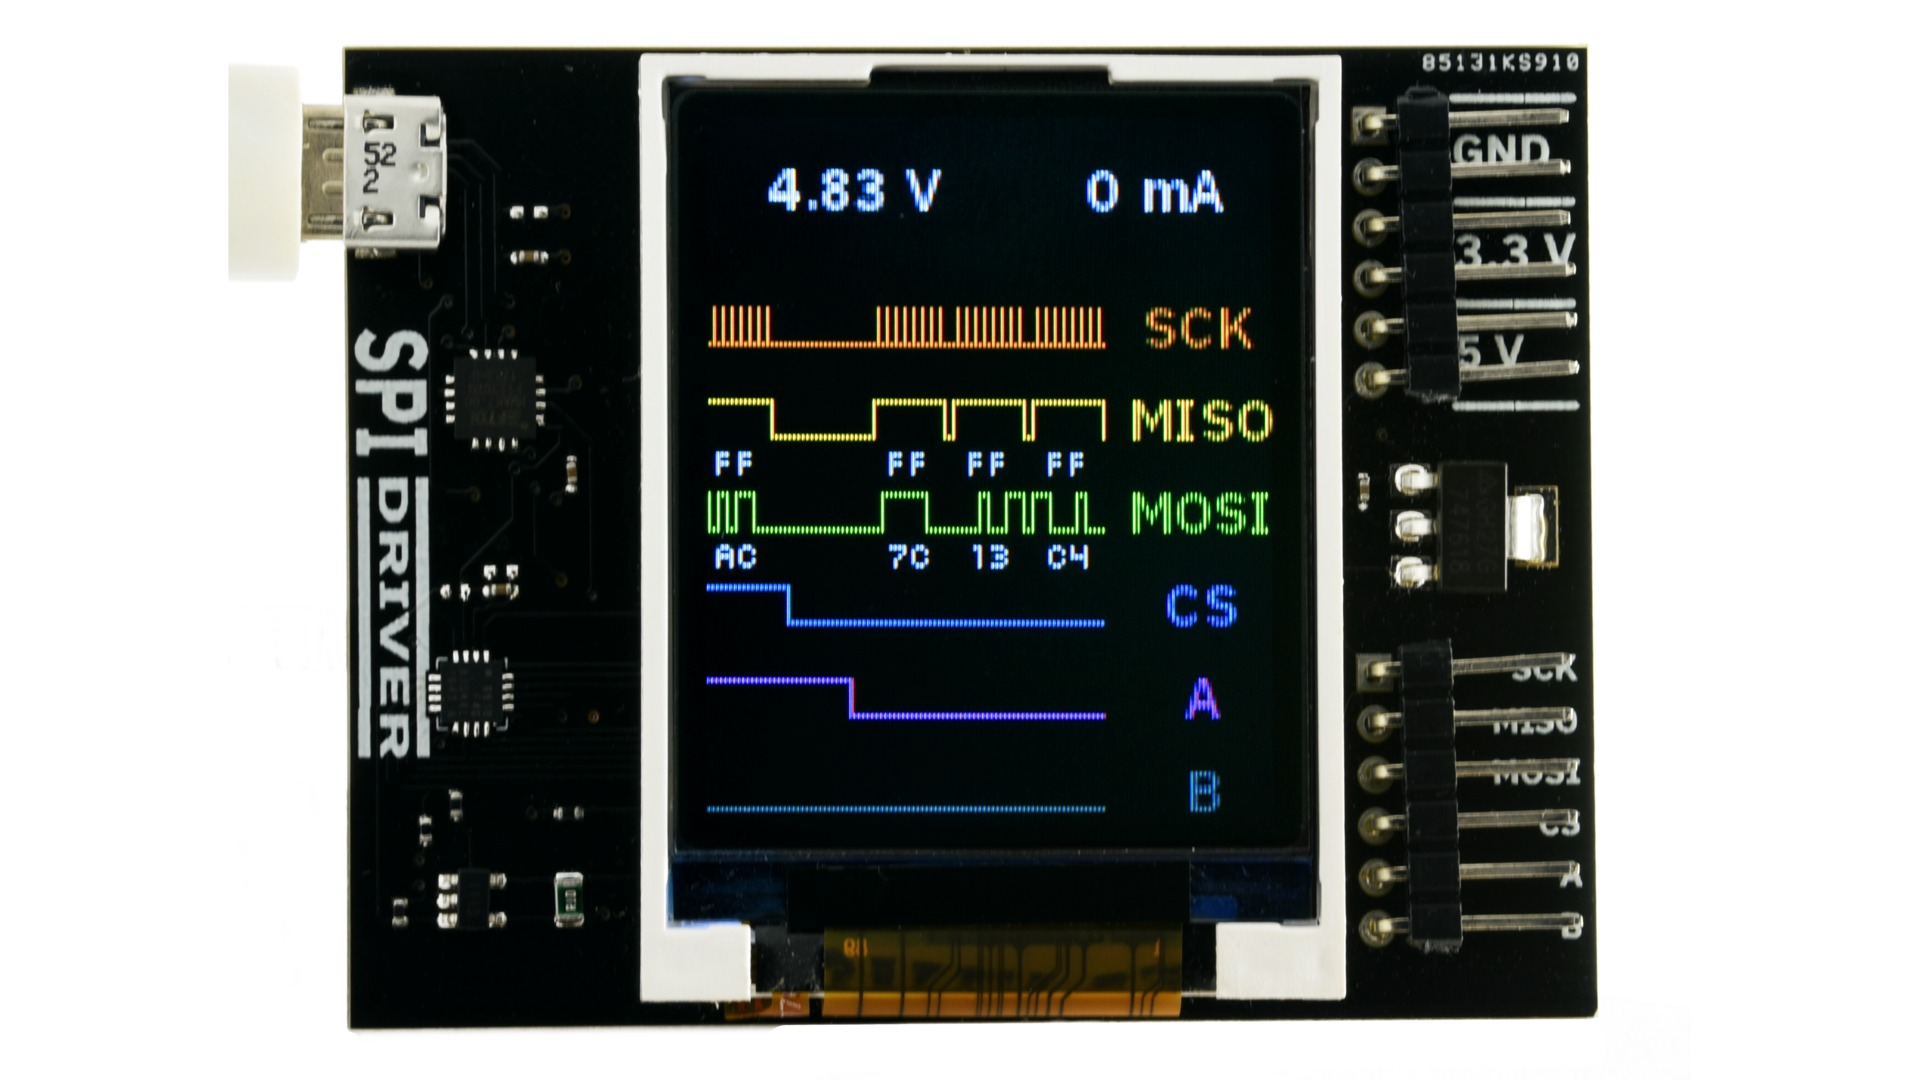
\includegraphics[width=1.00\textwidth]{img/spidriver/main}
Last updated on \today
\end{center}
\tableofcontents

\newpage

\setlength{\parindent}{0mm}
\setlength{\parskip}{1mm}
\setstretch{1.4}

\section{概论}

是一个易于使用,开源的工具,通過USB控制SPI设备.
它可以运行于 Windows, Mac, and Linux 平台上。
可以实时显示所有的SPI活動信息

\subsection{特性}
\begin{itemize}
\item {实时显示}: 精确显示
\item 高達500 K bps 的传送速率
\item {USB 电压监控}: 侦测USB电压供应问题, 低至0.01v
\item {目标设备电源监控}: 测量目标设备高侧电流, 精确至5 mA  
\item 兩個輔助輸出信號: A 和 B
\item 專門的電源輸出: 3.3v和5v 兩組電源和地綫
\item 信号线均与调线的颜色相同
\item 所有信号都是3.3 伏特, 兼容5 伏
\item 使用FTDI USB转串口芯片, 和Silicon Labs 汽车级 EFM8 控制器
\item 报告运行时间,温度和所有流量的CRC
\item 所有的传感器和信号都由一套简单的信号协议控制
\item 提供了在Windows, Mac, 和 Linux 上运行的GUI, 命令行, C/C++, and Python 2/3 软件支持工具 
\end{itemize}

\newpage
\section{开始}


当你第一次连接到USB端口, 屏幕会短暂闪白色后显示如下: 

\png{img/spidriver/spidriver-close}

按照下图所示的顺序连接六个颜色的信号线。 
\gap
\begin{center}
\begin{tabular}{ll}
\hline
\mach{SCK}  & 橙色 \\
\mach{MISO} & 黄色 \\
\mach{MOSI} & 绿色  \\
\mach{CS}   & 蓝色   \\
\mach{A}    & 紫色 \\
\mach{B}    & 灰色   \\
\hline
\end{tabular}
\end{center}
\gap

最上面为六条信号线。 剩下六条线为地线, 3.3V 和 5V 各两条。 
SPIDriver 持续测量USB输入电压和输出电流, 并显示在屏幕上方。 


\newpage
\section{软件安装}

所有的软件源代码在: 
\href{https://github.com/jamesbowman/spidriver}{repository}.
包含:

\begin{itemize}
\item Windows/Mac/Linux 图形界面工具
\item Windows/Mac/Linux 命令行工具
\item Python 2/3  绑定
\item Windows/Mac/Linux 之上的C/C++ 绑定
\end{itemize}

图形和命令行工具根据平台不同, 安装也不尽相同。
\subsection{Windows}\index{software!Windows}

这个安装
\href{https://spidriver.com/windows}{包}
包含了 图形界面和命令行工具.
以下的图标会出现在桌面上:

\png{img/spidriver/icon}

启动它就出现下述控制窗口

\png{img/spidriver/gui}

如果你只有一台串口设备, SPIDriver 会自动被选中。 

如果你有多台设备, 需要在上面的下拉菜单中选择COM 端口。 
一旦选中, 你就可以控制所有的信号线,并传输十六进制的数据

\index{spicl@\mach{spicl}}
命令行工具 \mach{spicl} 也已经安装. 例如, 可以展示如下信息:

\begin{lstlisting}
  C:\>"c:\Program Files\Excamera Labs\SPIDriver\spicl.exe" COM3 i
  uptime 1625  4.810 V  45 mA  23.3 C
\end{lstlisting}

关于命令行的语法, 请参考下述信息

\subsection{Linux}\index{software!Linux}

Linux上运行的图形化工具可以在此
\href{https://spidriver.com/linux}{spigui-linux64}  下载.
或者你也可以用如下所示的方法运行Python GUI
\index{spicl@\mach{spicl}}
要构建命令行工具, 克隆\href{https://github.com/jamesbowman/spidriver}{repository}, 然后:
\begin{lstlisting}
    $ cd spidriver/c
    $ make -f linux/Makefile
    $ ./build/spicl /dev/ttyUSB0 i
\end{lstlisting}
你会看到:

\begin{lstlisting}
    uptime 2285  4.812 V  45 mA  23.6 C
\end{lstlisting}

\subsection{MacOS}\index{software!Mac}

MacOS 的图形化工具可以在此
\href{https://spidriver.com/mac}{spigui-macos} 下载.
这是一个Mac的可执行文档, 下载后需要做:
\begin{lstlisting}
    $ cd Downloads
    $ chmod a+x spigui-macos
    $ ./spigui-macos
\end{lstlisting}

或者你也可以用如下所示的方法运行Python GUI.

\index{spicl@\mach{spicl}}
要构建命令行工具, 克隆\href{https://github.com/jamesbowman/spidriver}{repository}, 然后:


\begin{lstlisting}
    cd spidriver/c
    make -f linux/Makefile
    ./build/spicl /dev/cu.usbserial-DO00QS8D i
\end{lstlisting}

(substituting your actual SPIDriver's ID for \mach{DO00QS8D})
and you should see something like:
\begin{lstlisting}
    uptime 2285  4.812 V  45 mA  23.6 C
\end{lstlisting}

请注意使用的端口在 \mach{/dev/cu.usbserial-XXXXXXXX}, 这里 \href{https://pbxbook.com/other/mac-tty.html}{here} 有详细解释.

\section{APIs}
\subsection{Python 2 和 3}

SPIDriver 绑定可以通过\mach{pip} 安装:

\begin{lstlisting}
    pip install spidriver
\end{lstlisting}

然后从Python环境做:

\begin{lstlisting}
    >>> from spidriver import SPIDriver
    >>> s = SPIDriver("/dev/ttyUSB0") 
    >>> s.sel()                       
    >>> s.write([0x9f])               
    >>> list(s.read(3))              
    [239, 64, 24]
    >>> s.unsel()                     
    >>>
\end{lstlisting}

然后你会看到:
\png{img/spidriver/spidriver-flash}

使用wxPython 的图形界面工具可以如此运行:

\begin{lstlisting}
    python spigui.py
\end{lstlisting}

根据你所得到的安装包不同, 你会得到: 

\png{img/spidriver/spidriver-gui-linux}

更多例子在此: 
\href{https://github.com/jamesbowman/spidriver/tree/master/python/samples}{\mach{python/samples}} .

\subsection{C/C++}

SPIDriver 包含于一个单一头文件的唯一源文件中。 
他们在此\href{https://github.com/jamesbowman/spidriver/tree/master/c/common}{\mach{c/common}} .
使用下列的Python API 是非常直观的.

\newpage
\section{使用SPI Drive}

\subsection{The command-line tool \mach{spicl}}
\index{spicl@\mach{spicl}}

\mach{spicl} 在所有平台上都一样.

The first parameter to the command is the serial port, which depends on your operating system.
All following parameters are control commands. These are:

第一个参数是串口, 这取决于你的操作系统。 
所有随后的参数都是控制命令, 它们是:

\gap\begin{tabular}{ll}
\hline \\
  \mach{i}     & 打印状态信息(运行时间, 电压, 电流, 温度) \\
  \mach{s}     & SPI 开始 \\
  \mach{u}     & SPI 结束 \\
  \mach{w} $byte$\mach{,}...     & 写入字节到SPI \\
  \mach{r N}   & 从SPI读字节 \\
  \mach{a 0/1} & 设置A\\
  \mach{b 0/1} & 设置B\\
\hline \\
\end{tabular}
\gap

比如命令:

\begin{lstlisting}
  spicl /dev/ttyUSB0 s w 0x9f r 3 u
\end{lstlisting}

做了以下事情:

\gap\begin{tabular}{ll}
\hline \\
 \mach{s}       & SPI 开始 \\
 \mach{w 0x9f}  & 写字节 \mach{0x9f} \\
 \mach{r 3}     & 读出三个自己 \\
 \mach{u}       & SPI 结束\\
\hline \\
\end{tabular}

字节默认是十进制, 十六进制会以\mach{0x}开头。 

若要发送多个自己, 中间请用逗号隔开。 


\section{例子}
\subsection{ST7735R 1.8" LCD}\index{Examples!ST7735R}

ST7735R 是一个小型彩色LCD控制器, 其分辨率为160x128. 
它有个SPI-Like 的控制接口。 它并不适用MISO,而且需要额外一根控制线来区别命令字节和数据字节。 

它还需外部的重置信号获得稳定的启动。 


连接LCD 如下方式:

\pngw{img/spidriver/spidriver-lcd-1}{0.5}

\begin{center}
\gap\begin{tabular}{ccc}
\hline
SPIDriver&        & LCD     \\
\hline
3.3V     & 棕色 & LED     \\
SCK      & 橙色 & SCK     \\
MOSI     & 绿色  & SDA     \\
A        & 紫色 & A0      \\
B        & 灰色   & RESET   \\
CS       & 蓝色   & CS      \\
GND      & 黑色  & GND     \\
3.3V     & 红色    & VCC     \\
\hline \\
\end{tabular}
\end{center}

这里有一个Python的例子程序,展示在屏幕上显示一张图片。 
它需要 pillow 来做图片的装载, 所以你需要安装: 
\begin{lstlisting}
    pip install pillow
\end{lstlisting}

然后在SPIDriver的库中运行:

\begin{lstlisting}
    cd python/samples
    python st7735s.py -h /dev/ttyUSB0 grace.png
\end{lstlisting}

你可以把最后一个参数设置为任何的图形文件, 
脚本会缩放后显示它。 

\subsection{SPI Flash}\index{Examples!SPI flash}\index{flash}

要先在其手册中确定Flash的管脚输出, 现代的SPI Flash通常有下列类似的输出: 

\png{img/spidriver/spidriver-flash-0}
连接夹子到Flash芯片, 红色线在管脚1. 
下图为夹子连接到ESP8266板子上的Flash 芯片:


\png{img/spidriver/spidriver-esp1}
 
\index{ESP8266}
对于ESP8266, CPU 需要保持在重置状态, 以便保证在SPIDriver 驱动Flash芯片时不会产生竞争。 
连接SPIDrive 的A信号(紫色)到ESP8266的重置信号:
 
\png{img/spidriver/spidriver-esp2}

\png{img/spidriver/spidriver-flash-2}

连接夹子与SPIDriver 如下: 

\begin{center}
\gap\begin{tabular}{ccc}
\hline
SPIDriver&        & flash   \\
\hline
\mach{CS}         & 蓝色   & 1 \\
\mach{MISO}       & 黄色 & 2 \\
                  &        & 3 \\
\mach{GND}        & 黑色  & 4 \\
\mach{MOSI}       & 绿色  & 5 \\
\mach{SCK}        & 橙色 & 6 \\
                  &        & 7 \\
\mach{3.3V}       & 红色    & 8 \\
\hline \\
\end{tabular}
\end{center}

\index{JEDEC ID}

你可以用命令行工具确认3个字节的JEDEC ID:

\begin{lstlisting}
    $ spicl /dev/ttyUSB0 a 0 u s w 0x9f r 3 u
    0xc8,0x40,0x13
\end{lstlisting}

具体的ID 编码因制造商不同而不同。 它们通常列在Flash的手册上。 
第三个字节为Flash的大小(以位为单位), 所以上述的Flash是 
$2^{19} = 524288$ 字节, or 512K 字节.
如果你没有看到有效的ID, 你应该重新检查管脚, 确保夹子和所有的Flash管脚已经完全连接。 
这是一个Python的例子 
\href{https://github.com/jamesbowman/spidriver/blob/master/python/samples/flash.py>}{flash.py}
它用标准的SPI Flash 命令读写Flash的内容. 
若是没有其他选项,它会打印出来JEDEC ID作为确认: 

\begin{lstlisting}
    $ python flash.py -h /dev/ttyUSB0
    Got JEDEC ID: c8 40 13
    Flash size is 524288 bytes
\end{lstlisting}

你可以把所有的Flash内容读入一个文件中,使用 \mach{-r} 的选项:


\begin{lstlisting}
    $ python flash.py -h /dev/ttyUSB0 -r flashfile
    Got JEDEC ID: c8 40 13
    Flash size is 524288 bytes
    0/512 KBytes
    8/512 KBytes
    ...
    504/512 KBytes
\end{lstlisting}

相似的, \mach{-w} 选项擦除Flash并写入一个文件: 

\begin{lstlisting}
    $ python flash.py -h /dev/ttyUSB0 -w flashfile
    Got JEDEC ID: c8 40 13
    Flash size is 524288 bytes
    0/512 KBytes
    ...
    504/512 KBytes
\end{lstlisting}


许多Flash设备 , 如同上面的那个, 在ID的第三个字节报告它们的大小。 
然而, 有一些设备并不遵守上述规范。 
为了支持这些设备, 脚本的\mach{-s} 选项可以指定设备的大小, 而覆盖默认的计算结果。 


% 扩展连接器
% ------------------
% 
% 扩展连接器连接SPIDriver 信号到Arduino 标准 SPI 接口,
% 所以你可以使用Arduino的扩展板与SPIDriver 项链.
% 除了 电源 (地线, 3.3 V and 5 V) 它如下连接:
% 
% ========= ===========
% SPIDriver Arduino 管脚
% ========= ===========
% SCK       13
% MISO      12
% MOSI      11
% CS        8
% A         9
% B         10
% ========= ===========

\newpage
\section{注意事项}

\subsection{Port names}\index{USB ports}\index{port names}

SPIdriver 在不同的操作系统会有不同的串口名称。 
在Windows上, 它成为COM1, COM2, COM3 等等.
你可以使用 设备管理器或者\mach{MODE} 命令来显示所有已知的端口
\href{https://plugable.com/2011/07/04/how-to-change-the-com-port-for-a-usb-serial-adapter-on-windows-7/}{这篇文章}
描述了如何把一个设备设置为固定的端口.

在Linux平台, 它显示为\mach{/dev/ttyUSB0}, 1, 2 等.
实际的数字取决于设备加入的顺序。 
然而,它也有可能显示为如下: 

\begin{lstlisting}
    /dev/serial/by-id/usb-FTDI_FT230X_Basic_UART_DO00QS8D-if00-port0
\end{lstlisting}

\mach{DO00QS8D} 是SPIDriver的串行代码(它通常打印在SPIDriver的地步).
它长了一些,但是每次都是同一个名称。 

与此相似的是\textbf{Mac OS}, SPIDriver 出现为 \mach{/dev/cu.usbserial-DO00QS8D}.

\subsection{减少USB的延迟时间}

SPIDriver的性能可以通过设置USB的先吃时序到最小值1毫秒得以提高。 
这可以提高速度最高可达10倍。

在 \textbf{Linux} 平台设置:

\begin{lstlisting}
    setserial /dev/ttyUSB0 low_latency
\end{lstlisting}

在 \textbf{Windows} 或者 \textbf{Mac OS} 平台上, 参考
\href{https://projectgus.com/2011/10/notes-on-ftdi-latency-with-arduino/}{文章}.

\subsection{温度传感器}\index{temperature sensor}

温度传感器位于EFM8 控制器内。 它在出厂时已经校正到精确至2摄氏度。 
突然的温度上升表明其中的一个管脚(MOSI, SCK, CS, A, or B)与VCC 或地线短路

\subsection{原始协议}\index{protocol}
SPIDriver使用一个串口协议来发送和接受SPI命令。 
以此参数460800 baud, 8 bits, no parity, 1 stop bit (460800 8N1)连接到SPIDriver

\index{speed!serial}
许多SPIDriver commands 是ASCII,你可以从任何支持460800波特率的终端程序控制它。
比如输入 u 和 s 以切换CS 线, 键入 ? 显示状态信息。 
命令是: 


\gap\begin{tabular}{ll}
\hline
\mach{?}        & 状态信息 (参考下面)        \\
\mach{e} $byte$ & 回显 $byte$       \\
\mach{s}        & 选中        \\
\mach{u}        & 取消选中        \\
\mach{a} $byte$ & 设置A到0或1	\\
\mach{b} $byte$ & 设置B到0或1     \\
\mach{x}        & 从SPI Bus断开连接       \\
\mach{0x80-bf}  & 读取 1-64 字节       \\
\mach{0xc0-ff}  & 写入 1-64 字节        \\ \hline
\end{tabular}\gap

别入选中和传输2个字节\mach{0x12,0x34},取消选中, 主机发送  5 个字节.
命令 \mach{0x81} 是两字节读取,两个字节回到PC.

\begin{lstlisting}
s
0x81
0x12
0x34
u
\end{lstlisting}


状态信息总是80个字符, 以空白符填充。 例如:


{\scriptsize
\begin{framed}\begin{Verbatim}
[spidriver1 DO00QS8D 000007219 4.807 045 25.4 1 1 1 49c1                       ]
\end{Verbatim}
\end{framed}}

信息中的位域由空白分割:

\gap\begin{tabular}{ll}
\hline
spidriver1      & 固定字符 \\
serial          & 设备序列号 \\
uptime          & 运行时间 0-999999999, 以秒为单位 \\
voltage         & USB总线电压, 以伏特为单位 \\
current         & 设备总线电流, 以 mA 毫安为单位 \\
temperature     & 设备温度,以摄氏度为单位 \\
CS              & CS 线状态 \\
A               & A 线状态 \\
B               & B 线状态 \\
crc             & 所有输入和输出字节的16-bit CRC  (CRC-16-CCITT)  \index{CRC}\\
\hline
\end{tabular}\gap

\newpage
\subsection{规范}\label{electrical-characteristics}

\subsubsection*{DC 特性}
\vspace{10 pt}
{\renewcommand{\arraystretch}{1.2}% for the vertical padding

\begin{tabularx}{\linewidth}{XC{40pt}C{40pt}C{40pt}C{40pt}}
\heavyline
& 最小 & 典型 & 最大 & 单位 \\ \heavyline

电压精度              && 0.01 && V            \\ \hline
电流精度         && 5 && mA              \\ \hline
温度精度          && $\pm$ 2 && $^{\circ}$C            \\ \hline
MISO & & & & \\
\hspace{10pt}低压 & & & 0.6 & V \\
\hspace{10pt}高压 & 2.7 &   & 5.8 & V \\ \hline
输出信号电流 (SCK, MOSI, CS, A, B)  &&& 8 & mA \\ \hline
输出电流        & & & 470 & mA                  \\ \hline
电流消耗   & & 25 & & mA                   \\ \hline

\end{tabularx}}
\vspace{10 pt}

\subsubsection*{AC 特性}
\vspace{10 pt}

{\renewcommand{\arraystretch}{1.2}% for the vertical padding
\begin{tabularx}{\linewidth}{XC{40pt}C{40pt}C{40pt}C{40pt}}
\heavyline
& 最小 & 典型 & 最大 & 单位 \\ \heavyline

SPI 速度                     &495& 500 &505& Kbps   \index{speed!SPI}\\ \hline
运行时间精度               && 150 && ppm           \index{uptime}\\ \hline
运行时间回滚               && 31.7 && years        \\ \hline
启动时间 & & & 200 & ms \\ \hline
\end{tabularx}}
\vspace{10 pt}

\section{支援信息}

技术和产品支援可以在此
\href{mailto:support@spidriver.com}{support@spidriver.com}找到

SPIDriver 由
\href{https://excamera.com}{Excamera Labs} 创建和维护.

\newpage
\raggedright
\addcontentsline{toc}{section}{Index}
\renewcommand{\indexname}{Index}
\printindex

\end{document}
